\documentclass{standalone}
\usepackage{tikz}
\usepackage{amsmath}
\usetikzlibrary{arrows.meta}

\begin{document}
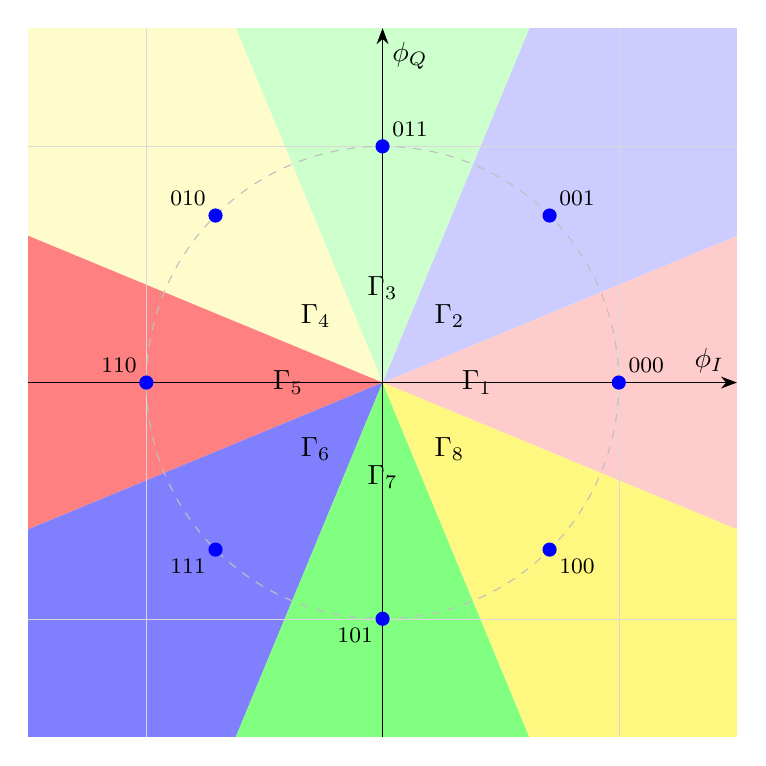
\begin{tikzpicture}[scale=3]

    % Fill the four quadrants with different colors
    \fill[red!20] (0,0) -- ({1.5},{1.5*tan(pi/8 r)}) -- ({1.5},{-1.5*tan(pi/8 r)}) -- (0,0) -- cycle;
    \fill[blue!20] (0,0) -- ({1.5}, {1.5*tan(pi/8 r)}) -- (1.5, 1.5) -- ({1.5*tan(pi/8 r)}, 1.5)-- (0,0) -- cycle;
    \fill[green!20] (0,0) -- ({1.5*tan(pi/8 r)}, 1.5) -- (-{1.5*tan(pi/8 r)}, 1.5) -- (0,0) -- cycle;
    \fill[yellow!20] (0,0) -- ({-1.5}, {1.5*tan(pi/8 r)}) -- (-1.5, 1.5) -- (-{1.5*tan(pi/8 r)}, 1.5)-- (0,0) -- cycle;
    \fill[red!50] (0,0) -- ({-1.5},{1.5*tan(pi/8 r)}) -- ({-1.5},{-1.5*tan(pi/8 r)}) -- (0,0) -- cycle;
    \fill[blue!50] (0,0) -- ({-1.5}, {-1.5*tan(pi/8 r)}) -- (-1.5, -1.5) -- ({-1.5*tan(pi/8 r)}, -1.5)-- (0,0) -- cycle;
    \fill[green!50] (0,0) -- ({-1.5*tan(pi/8 r)}, -1.5) -- ({1.5*tan(pi/8 r)}, -1.5) -- (0,0) -- cycle;
    \fill[yellow!50] (0,0) -- ({1.5}, {-1.5*tan(pi/8 r)}) -- (1.5, -1.5) -- ({1.5*tan(pi/8 r)}, -1.5)-- (0,0) -- cycle;
    
    % Add region labels (Gamma)
    \node at (0.4, 0) {$\Gamma_1$};
    \node at ({0.4*cos(pi/4 r)},{0.4*sin(pi/4 r)}) {$\Gamma_2$};
    \node at (0,0.4) {$\Gamma_3$};
    \node at (-{0.4*cos(pi/4 r)},{0.4*sin(pi/4 r)}) {$\Gamma_4$};
    \node at (-0.4,0) {$\Gamma_5$};
    \node at (-{0.4*cos(pi/4 r)},{-0.4*sin(pi/4 r)}) {$\Gamma_6$};
    \node at (0,-0.4) {$\Gamma_7$};
    \node at ({0.4*cos(pi/4 r)},{-0.4*sin(pi/4 r)}) {$\Gamma_8$};

    \draw[help lines,gray!30] (-1.5,-1.5) grid (1.5,1.5);
    
    \draw[-{Stealth[scale=1.2]}] (-1.5,0) -- (1.5,0) node[above, xshift=-10pt] {$\phi_I$};
    \draw[-{Stealth[scale=1.2]}] (0,-1.5) -- (0,1.5) node[right, yshift=-10pt] {$\phi_Q$};
    
    \draw[dashed,gray!50] (0,0) circle (1);
    
    % Constellation points
    \fill[blue] (1, 0) circle (0.03);
    \node[above right] at (1, 0) {\footnotesize 000};

    \fill[blue] ({1/sqrt(2)},{1/sqrt(2)}) circle (0.03);
    \node[above right] at ({1/sqrt(2)},{1/sqrt(2)}) {\footnotesize 001};
    
    \fill[blue] (0, 1) circle (0.03);
    \node[above right] at (0, 1) {\footnotesize 011};
    
    \fill[blue] ({-1/sqrt(2)},{1/sqrt(2)}) circle (0.03);
    \node[above left] at ({-1/sqrt(2)},{1/sqrt(2)}) {\footnotesize 010};

    \fill[blue] (-1, 0) circle (0.03);
    \node[above left] at (-1, 0) {\footnotesize 110};
    
    \fill[blue] ({-1/sqrt(2)},{-1/sqrt(2)}) circle (0.03);
    \node[below left] at ({-1/sqrt(2)},{-1/sqrt(2)}) {\footnotesize 111};
    
    \fill[blue] (0, -1) circle (0.03);
    \node[below left] at (0, -1) {\footnotesize 101};
    
    \fill[blue] ({1/sqrt(2)},{-1/sqrt(2)}) circle (0.03);
    \node[below right] at ({1/sqrt(2)},{-1/sqrt(2)}) {\footnotesize 100};

\end{tikzpicture}
\end{document}